%!TEX root = ../main.tex
%
% 光の干渉
%


\section{光の干渉}

\subsection{波としての光の性質}

前の章で述べたように光の正体は電磁波という「波」です。光の持つ反射や屈折等の性質を調べても光が波の性質を
持つ事は実感できませんが、光の経路をスリット等を使って分けた後に再び重ね合わせると水の波の実験で見た様な
「干渉」という波が持つ特有の現象を観察することができます。

この章の実験では干渉をおこしやすい性質を持つレーザー光を用い、ダブルスリットや回折格子で光がどのように
して干渉をおこすのか調べ、その結果からレーザー光の波長を求めます。

\subsection{単スリット}

\begin{wrapfigure}[6]{r}{7cm}
\vspace*{-0.8cm}
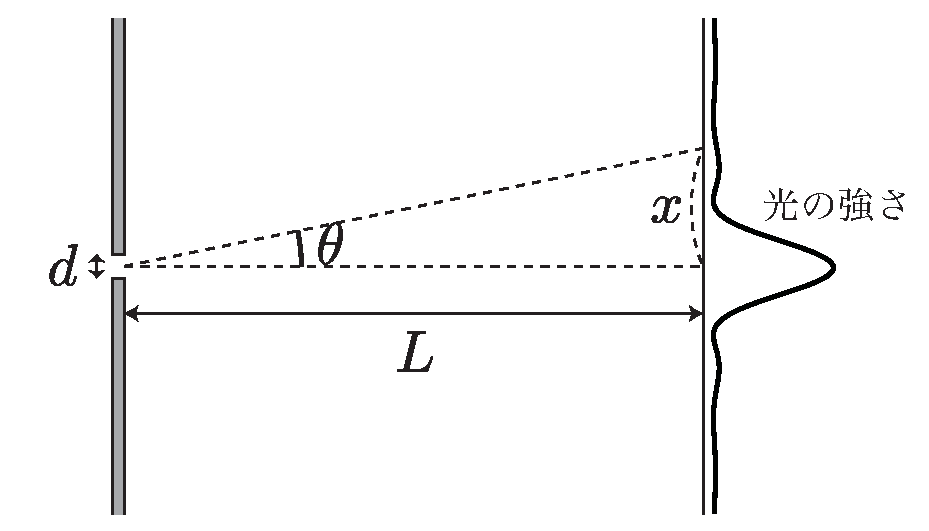
\includegraphics[scale=0.5]{03_Interference/one-slit.eps}
\end{wrapfigure}


まず、幅$d$の単スリットがある障壁を考えてみましょう。この障壁に垂直に入射し、ス
リットを通った波長$\lambda$の光の強度は次の式のようになります。
\[
I(\theta)=I_0
\left|
\frac{\sin\left(\frac{\pi}{\lambda}d\sin\theta\right)}{\frac{\pi}{\lambda}d\sin\theta}
\right|^2
\]

この式から、最初に光が弱くなる($I(\theta)=0$となる)のは、
\begin{equation}
d\sin\theta=\lambda
\label{dark line}
\end{equation}
の時になります。続いて、 
\[
d\sin\theta=2\lambda,~3\lambda,\cdots
\]
のように、波長の整数倍の条件を満たす方向で光が弱まり、暗線が見えます。

また、$\theta=0$の時に光の強度は最大となりますが、他の明線(明るさのピーク)の
条件は一般に求めるのは難しく、
\[
d\sin\theta \simeq \frac{5}{2}\lambda,~\frac{7}{2}\lambda,\cdots
\]
の条件を満たす方向付近に明線が現れます。

%\bigskip
%
%\hspace*{-\parindent}
%※ $\theta=0$の時は、光の強度が最大になることに注意


ここで、図のように、障壁から距離$L$の所
にスクリーンを置きます。スクリーン上で、ス
リットの中心から直進して到達する点から、最初
に光が弱くなる所までの距離を$x$とすると、光の
強度が最初に弱まる所を表わす(\ref{dark line})の式は、$x$に 
比べて$L$が充分に大きい場合には、($\sin\theta\simeq x/L$として)
\begin{equation}
\frac{d\,x}{L}=\lambda
\label{approx dark line}
\end{equation}
と近似して書くことができます。(\ref{approx dark line})
の式から、$d$, $x$, $L$を測定すれば、光の波長$\lambda$が求められます。
%$\Rightarrow${\bf [実験 3-1]}


\subsection{ダブルスリット}


\begin{wrapfigure}[7]{r}{7cm}
%\vspace*{-0.8cm}
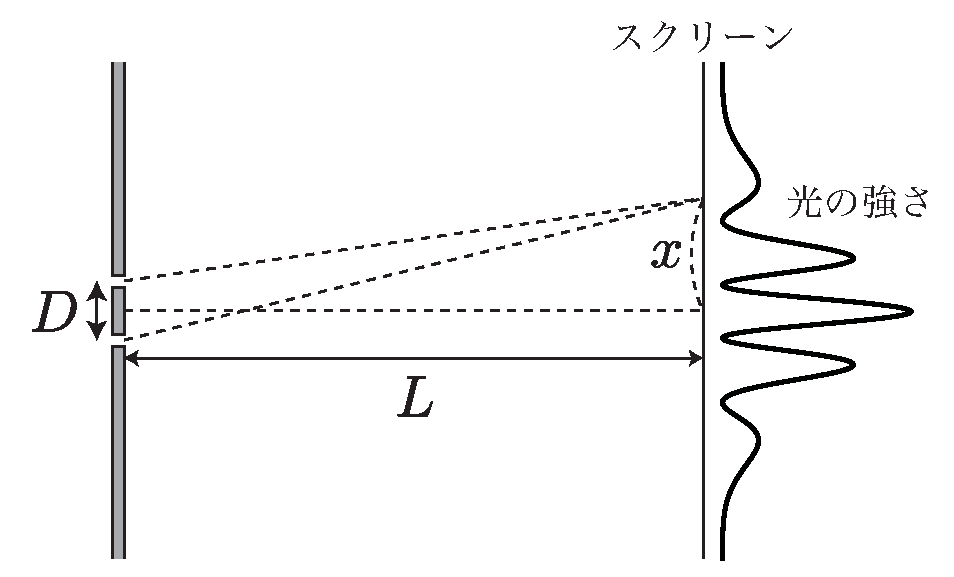
\includegraphics[scale=0.5]{03_Interference/two-slits.eps}
\end{wrapfigure}


まず、細いスリットが二本開いているダブルスリットを考えましょう。
2本のスリットの間隔を$D$とし、スリットの幅は無視できるとします。障壁とスク
リーンの距離を$L$とすると、スクリーン上で中心からの水平
距離が$x$である点における「左スリットから入った光と右ス
リットから入った光が通ってきた道のりの差」=光路差は、
\begin{eqnarray}
光路差&=&\sqrt{L^2+\left(x+\frac{D}{2}\right)^2}
-\sqrt{L^2+\left(x-\frac{D}{2}\right)^2}\nonumber\\
&\simeq& \frac{x\,D}{L}\nonumber
\end{eqnarray}
となります。($x$に比べて$L$が充分に大きい場合。)

光が最も強くなるのは、$x=0$の所になります。それ以降は、
\[
\frac{x\,D}{L}=\lambda,~2\lambda,~3\lambda,\cdots
\]
となる所(光路差がちょうど光の波長の整数倍になる所)で同位相の波の重ね合わせ効果で
光が強められ明線が現れます。$\Rightarrow${\bf [実験 3-1]}

一方、逆位相で光が弱められて暗線が見えるのは、
\[
\frac{x\,D}{L}=\frac{1}{2}\lambda,~\frac{3}{2}\lambda,~\frac{5}{2}\lambda,\cdots
\]
のとき、すなわち、位相が半波長分ずれるときになります。 

\begin{center}
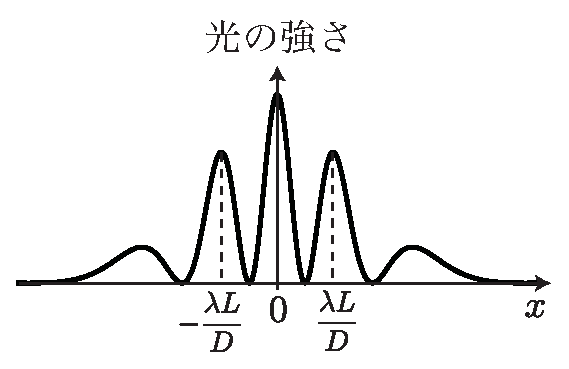
\includegraphics[scale=0.7]{03_Interference/two-slits-int.eps}
\end{center}


\subsection{回折格子}

\begin{wrapfigure}[10]{r}{7cm}
\vspace*{-0.5cm}
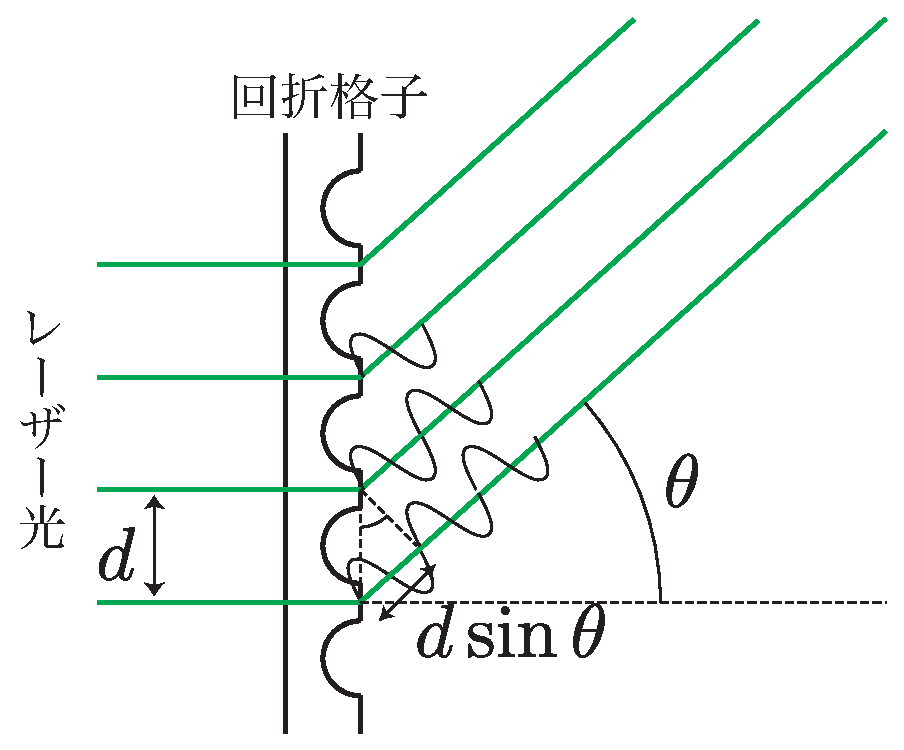
\includegraphics[scale=0.5]{03_Interference/grating.eps}
\end{wrapfigure}


回折格子とはガラス板やプラスチックフィルムに1mmあたり数百本もの細かい溝などの構造を等間隔で刻んだものです。
グレーチングやレプリカフィルム等とも呼ばれます。
細かい構造によって、光が透過する部分と遮られる部分が交互に繰り返し、透過した多数の光どうしが干渉した結果、
波長ごとに光が強められる方向が決まります。数が非常に多いスリットと考えても良いでしょう。

格子の間隔が$d$である回折格子に垂直に光を当てたとき、角度$\theta$で出て行く光どうしの光路差はすべて
\[
d\sin\theta
\]
となるので、この長さが波長の整数倍($\lambda,2\lambda,3\lambda,\cdots$)になるときに光は強め合います。
また、この長さが波長の半整数倍($\frac{1}{2}\lambda,\frac{3}{2}\lambda,\frac{5}{2}\lambda,\cdots$)
のときは光が弱め合う条件となりますが、
回折格子の場合は多数の光どうしで干渉するので、強め合う条件以外の方向に光は出て行くことはほとんどありません。
この結果、レーザーなどの点状の光源を用いた場合、干渉縞は明るい点の列となって現れます。$\Rightarrow${\bf [実験 3-2]}

回折格子からスクリーンまでの距離を$L$、スクリーン上で中心からの水平距離を$x$とすると、
\[
\sin \theta = \frac{x}{\sqrt{x^2+L^2}}
\]
と表され、$x$に比べて$L$が非常に大きい場合は、
\[
\sin \theta = \frac{x}{\sqrt{x^2+L^2}} \simeq \frac{x}{L}
\]
と近似できますので、これらを用いて明線(明点)の位置を決定したり、逆に明線の位置から
光の波長を求めることができます。






\newpage

\jikken

\begin{itemsquarebox}[c]{\bf 実験用具}
He-Neレーザー光源(赤色)、半導体レーザー光源(緑色)、架台、単スリット板、ダブルスリット板、
回折格子、CD、定規又は巻尺
\end{itemsquarebox}

\bigskip

%\subjikken{単スリットを用いた干渉縞の観察}

%\begin{enumerate}
%
%\item レーザー光源装置を架台の上に設置し、設置したスクリーン(方眼紙を使用)の
%中央に、レーザー光が当たるように高さを調節します。
%
%\item レーザー光源と方眼紙の距離を1 [m]以上離して設置しておきます。
%
%\item レーザー光源のビームの出口にある切り込みに、単スリット板を設置し、このス
%リットを通ったレーザー光により、スクリーン上に生じる干渉模様を観察しましょ
%う。干渉縞の最初の暗点と中心の明点の距離$x$、スリット板からスクリーンまで
%の距離$L$を測定し、スリットの幅$d$を考慮して、レーザー光の波長をそれぞれの
%スリット板について計算しましょう。
%
%
%\end{enumerate}

\subjikken{ダブルスリットを用いた干渉縞の観察}

\begin{enumerate}

\item レーザー光源装置を架台の上に設置し、設置したスクリーン(方眼紙を使用)の
中央に、レーザー光が当たるように高さを調節します。

\item レーザー光源と方眼紙の距離を1 [m]以上離して設置しておきます。

\item レーザー光源の前にスリットの間隔が0.1 [mm]および
0.2 [mm]の ダブルスリット板を設置し、このス
リットを通ったレーザー光により、スクリーン上に生じる干渉模様を観察しましょ
う。

\item 干渉縞の中心の明点と2番目の明点との距離$x$ [mm]、スリット板からスクリーンまで
の距離$L$ [mm]を測定し、スリットの幅$d$ [mm]を考慮して、
赤色と緑色のレーザー光の波長をそれぞれの
スリット板について計算しましょう。


\end{enumerate}



\bigskip

\subjikken{回折格子による干渉実験}

縦方向に一定間隔で細かい筋がたくさんついた回折格子を通すと、スクリー
ン上に写し出される干渉模様はどのようになるでしょうか。ダブルスリットでの干渉縞
と比較してみましょう。回折格子についてもダブルスリットのときと同様の実験を行い、
レーザー光の波長を求めてみましょう。

\bigskip


%\subjikken{ピンホールによる干渉実験}
%
%ピンホールや方眼回折格子の場合にはどのような干渉縞ができるでしょうか。
%今までの結果から予想して観察してみましょう。

\subjikken{CDのトラックピッチの測定}

CDには非常に細かい出っ張り(ピット)が刻まれていて、そこに音楽などのデジタルデータが記録されています。
ピットによって反射された光は回折格子と同様の原理で干渉をおこします。
CDにレーザー光線を反射させ、
その干渉縞(明点)の間隔およびCDとスクリーンまでの距離を測定し、
レーザー光線の波長からCDのピット列の間隔(トラックピッチ)を求めてみましょう。


\bigskip


\hspace*{-\parindent}
※ {\bf 注意}:レーザー光源を直接目に入れてはいけません。(ビームの出口をのぞき込まな
いこと。他人の顔の方向にビームを向けないこと。) また、鏡面反射を起こ
すもの(鏡、腕時計など)をビーム付近に近づけないようにしましょう。